\section*{Introduction}
\setcounter{figure}{0}

Let's first introduce the general term of data science. It is a new and important discipline that can be viewed as:
\begin{itemize}
  \item An amalgamation of classical disciplines such as statistics, data mining, databases, and distributed systems,
  \item With additional new challenges constantly emerging and making the field highly dynamic and appealing.
\end{itemize} 
The problems grow in terms of size ("Big data") and complexity of the questions to be answered. But the basic job can be summarized as:
\begin{itemize}
  \item Input: data $\Rightarrow$ Processed by data scientist (with tools) $\Rightarrow$ Output: value
  \item Where the skills of a data scientist are the combination of open mind, human interest, analytical skills, creativity, business-benefiting weighting, $\dots$
  \item Or in other terms as can be seen in \ref{fig:0_skillset}
\end{itemize}

\begin{figure}[H]
  \centering
  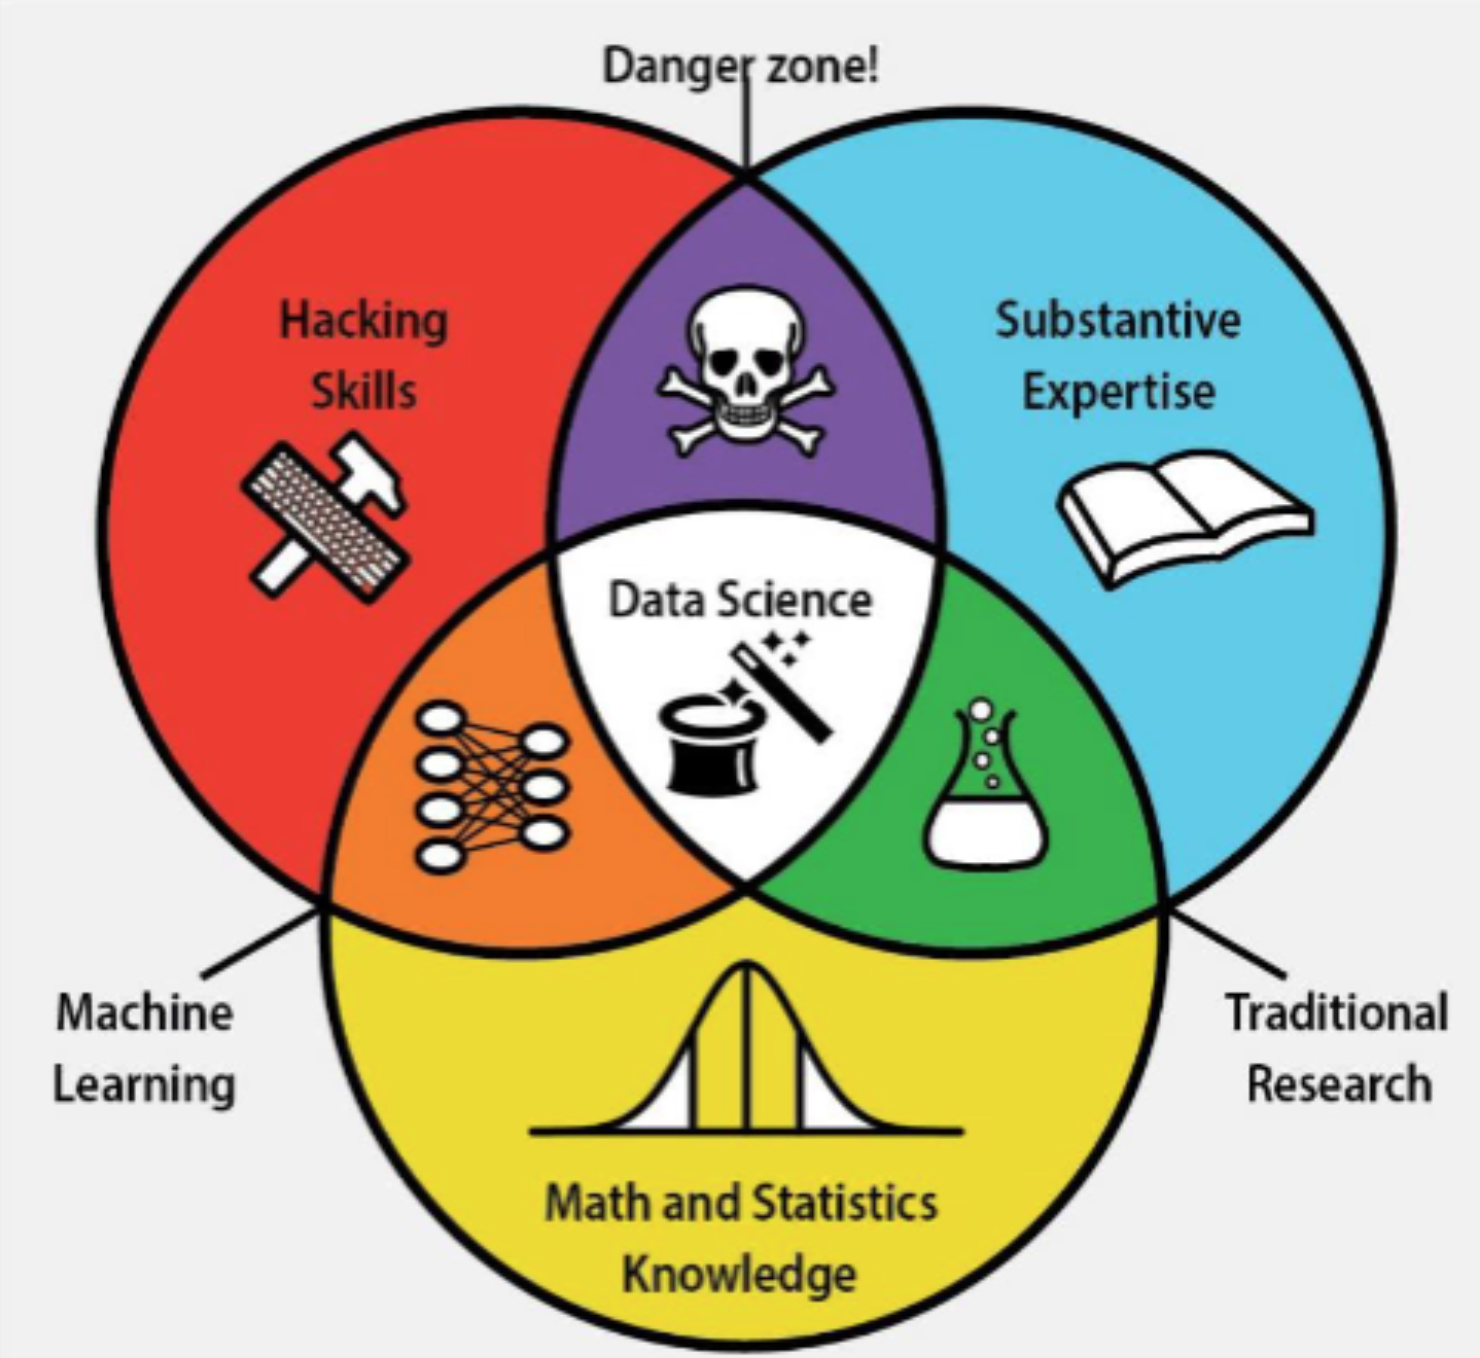
\includegraphics[width=0.4\textwidth]{assets/intro/data_scientist_skillset.png} 
  \begin{itemize}
    \item Data science: due to its interdisciplinary nature requires an intersection of the following abilities (H + M + S)
    \item Hacking skills (H): necessary for working with massive amounts of electronic data that must be acquired cleaned, and manipulated
    \item Math and statistics knowledge (M): to choose appropriate methods and tools to extract insight from data
    \item Substantive expertise in a scientific field (S): crucial for generating motivating questions and hypotheses and interpreting the results
    \item Traditional research: in the intersection of M and S
    \item Machine learning: combines H with M, but doesn't require scientific motivation
    \item !Danger zone: H and S combined without rigorous methods can beget incorrect analyses
  \end{itemize}
  \caption{Skillset of a data scientist}
  \label{fig:0_skillset}
\end{figure}

With the growing importance of data and digitalization, organizations are looking for data scientists, who may outnumber computer scientists in the future. Important is the ability to handle data in any form, so basically the need for an all-around skilled "data wizard". This importance can be further highlighted when looking at the tech development over the past 20 to 30 years. While the hardware got tremendously cheaper, faster, and more compact (20 times faster for MIP = mixed integer programs), also software has progressed in terms of speed (50 times faster for MIP). Interesting to look at is also the aspect of automation.

Dimensions of data science are:
\begin{itemize}
  \item The different types of data (structured or unstructured, text, images, events, $\dots$)
  \item The different types of tasks (supervised or unsupervised, $\dots$)
  \item Human versus machine (Who does what?)
  \item Algorithm versus visualization (What is needed?)
  \item Flexibility versus usability
  \item Scalability versus quality (exact versus heuristics)
  \item Responsibility versus utility (accuracy and precision versus fairness, privacy, transparency, $\dots$)
\end{itemize}

Besides raw data science, interesting to look at is also the connection to process science. The interplay between process and data science (PADS) leads to the term process mining. Imagine the connection as shown in \ref{fig:0_pads}.

\begin{figure}[H]
  \centering
  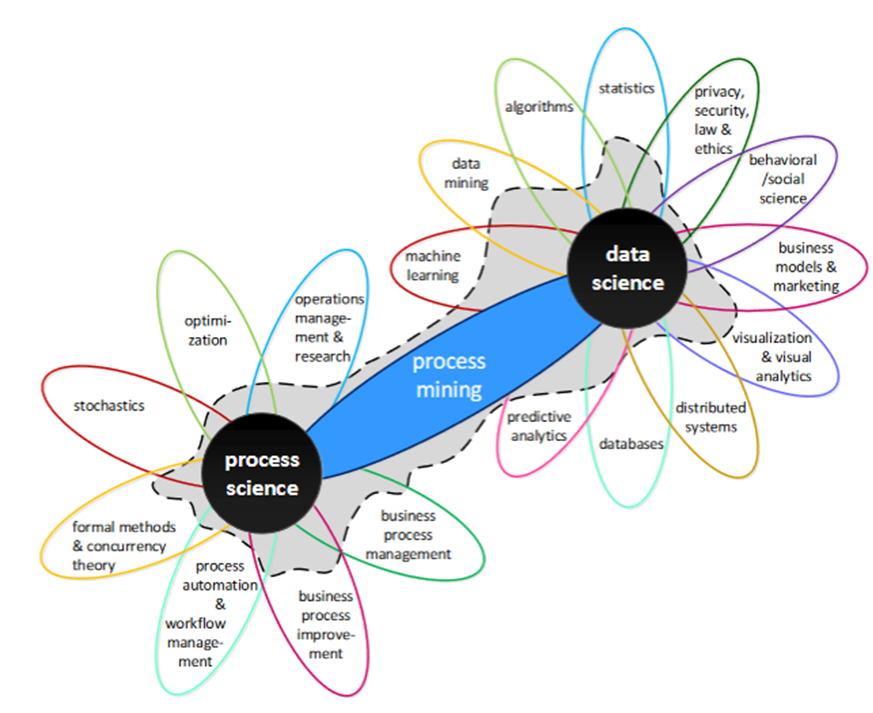
\includegraphics[width=0.75\textwidth]{assets/intro/pads.png} 
  \caption{Interplay between process science and data science}
  \label{fig:0_pads}
\end{figure}

As the final part of the introduction, we will now see the general covered topics in this course:
\begin{itemize}
  \item Basic data exploration and visualization
  \item Decision trees, regression, support vector machines
  \item Neural networks, evaluation of supervised learning problems, clustering
  \item Frequent items sets, association rules, sequence mining, process mining, text mining
  \item Data preprocessing/quality and binning, visual analytics and information visualization
  \item Responsible data science
  \item Big data technologies
\end{itemize}

